\documentclass{article}

\input{../../eq2845_commands.tex}

\begin{document}

\begin{center}
  \textbf{
    \LARGE HW3 \\
    \large EQ2845 -- Information Theory \& Source Coding \\
           Lukas Bjarre -- \mail{lbjarre@kth.se}
  }
  \rule{0.75\textwidth}{0.4pt} \\
\end{center}

\section{Q1: General Huffman questions}

\subsection{Lower bound of $D$ in prefix-free code}
For a $D$-ary prefix-free code Kraft's inequality gives us that 
\begin{equation}
  \sum_{i=1}^n D^{-l_i} \leq 1
  \label{eq:kraft}
\end{equation}
Inserting the given codeword lengths and trying for a some different integer values for $D$
shows that $D=3$ results in the left hand side being $\frac{26}{27}$,
which is the lowest integer value for which the inequality is upheld.

In the case of an uniquely decodable code we know that McMillan's inequality places the same
lower bound for this uniquely decodable code as the prefix-free code.
The lower bound is simply the same.

\subsection{2-ary Huffman codes}
Running the Huffman algorithm on the message probabilities gives the following tree:
\begin{figure}[!ht]
  \centering
  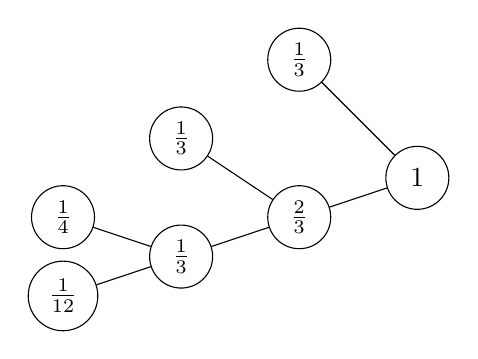
\begin{tikzpicture}[
    x=1.5cm,
    y=1cm,
    every node/.style={
      draw,
      circle,
      minimum size=0.8cm
    }
  ]
    \node (leaf1) at (2, 0) {$\frac{1}{3}$};
    \node (leaf2) at (1, -1) {$\frac{1}{3}$};
    \node (leaf3) at (0, -2) {$\frac{1}{4}$};
    \node (leaf4) at (0, -3) {$\frac{1}{12}$};
    \node (comb1) at (1, -2.5) {$\frac{1}{3}$};
    \node (comb2) at (2, -2) {$\frac{2}{3}$};
    \node (root) at (3, -1.5) {$1$};

    \draw[-] (leaf3) to (comb1);
    \draw[-] (leaf4) to (comb1);
    \draw[-] (leaf2) to (comb2);
    \draw[-] (comb1) to (comb2);
    \draw[-] (leaf1) to (root);
    \draw[-] (comb2) to (root);
  \end{tikzpicture}
  \caption{Huffman 2-ary tree for the random message $U$.}
  \label{fig:hufftree1}
\end{figure}

The different Huffman codes created by this tree
depends on which direction in the tree we represent with $0$ and $1$.
The two different codes are written out in \cref{tab:huffcodes}
together with the lengths and the optimal Shannon length.
We can see that the third codeword is longer than the Shannon length.
\begin{table}[!ht]
  \centering
  \renewcommand{\arraystretch}{1.2}
  \caption{All possible Huffman codes}
  \begin{tabular}{ccccc}
    $p_i$ & $c_{1,i}$ & $c_{2,i}$ & $\ceil{\log_2\frac{1}{p_i}}$ & $l_i$\\\hline
    $\frac{1}{3}$ & 0 & 1 & 2 & 1 \\
    $\frac{1}{3}$ & 10 & 01 & 2 & 2 \\
    $\frac{1}{4}$ & 110 & 001 & 2 & 3\\
    $\frac{1}{12}$ & 111 & 000 & 4 & 3 
  \end{tabular}
  \label{tab:huffcodes}
\end{table}

\subsection{Huffman code}
The resulting Huffman tree is presented in \cref{fig:hufftree2}
\begin{figure}[!ht]
  \centering
  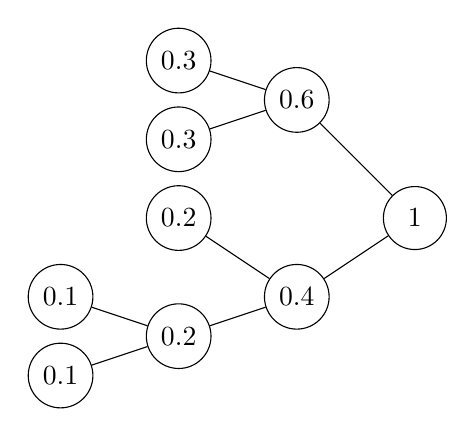
\begin{tikzpicture}[
    x=1.5cm,
    y=1cm,
    every node/.style={
      draw,
      circle,
      minimum size=0.8cm
    }
  ]
    \node (leaf1) at (1, 0) {$0.3$};
    \node (leaf2) at (1, -1) {$0.3$};
    \node (leaf3) at (1, -2) {$0.2$};
    \node (leaf4) at (0, -3) {$0.1$};
    \node (leaf5) at (0, -4) {$0.1$};

    \node (comb1) at (1, -3.5) {$0.2$};
    \node (comb2) at (2, -3) {$0.4$};
    \node (comb3) at (2, -0.5) {$0.6$};
    \node (root) at (3, -2) {$1$};

    \draw[-] (leaf5) to (comb1);
    \draw[-] (leaf4) to (comb1);
    \draw[-] (leaf3) to (comb2);
    \draw[-] (comb1) to (comb2);
    \draw[-] (leaf1) to (comb3);
    \draw[-] (leaf2) to (comb3);
    \draw[-] (comb2) to (root);
    \draw[-] (comb3) to (root);
  \end{tikzpicture}
  \caption{Huffman tree for the distribution $\mathbf{p}$.}
  \label{fig:hufftree2}
\end{figure}

We can see from the leaf node depths that the codewords will have lengths 2, 2, 2, 3, and 3.
The average length of this code is
\begin{equation}
  \begin{aligned}
    \expect{L}
    &= \sum_{i=1}^5 p_i l_i \\
    &= 0.3 \cdot 2 + 0.3 \cdot 2 + 0.2 \cdot 2 + 0.1 \cdot 3 + 0.1 \cdot 3 \\
    &= 2.2
  \end{aligned}
\end{equation}

A code with the same average codeword length as the entropy implies that
\begin{equation}
  \sum_{i=1}^5 p_i \log p_i = \sum_{i=1}^5 p_i l_i \\
\end{equation}
A simple way to ensure this is to set $l_i = \log p_i$ for all $i$.
Also note that we want to have integer lengths, so all probabilities need to be inverse powers of two
for a 2-ary code.
An example of message that fullfills this is
\begin{equation}
  \textbf{p'} = \left( \frac{1}{2},\,\frac{1}{4},\,\frac{1}{8},\,\frac{1}{16},\,\frac{1}{16} \right)
\end{equation}

\subsection{Possible Huffman codes}
$\mathbf{l}_1$ is a Huffman code.
\Cref{fig:hufftree1} with the bottom leafnodes is an example of such a Huffman code.

$\mathbf{l}_2$ is not a valid Huffman code,
since one of the codewords of length 2 can be reduced to one of length 1
without loosing any decodability.

In gerneral we know that for $D$-ary Huffman codes
the $D$ least likely messages are coded with codewords of the same length.
We can on this basis exclude $\mathbf{l}_3$ as a possible ternary Huffman code
since it has four different codeword with the highest length.

$\mathbf{l}_4$ is a possible Huffman code.
\Cref{fig:hufftree3} shows a possible realisation of this Huffman tree.
\begin{figure}[!ht]
  \centering
  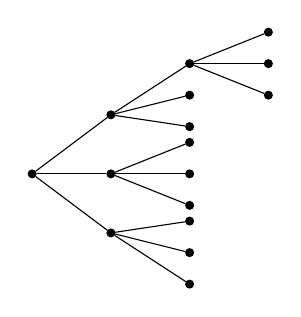
\begin{tikzpicture}[
    x=1cm,
    y=0.5cm,
    every node/.style={
      draw,
      circle,
      fill=black,
      inner sep=0pt,
      text width=0.1cm
    }
  ]
    \node (root) at (0, 0) {};
    \node (lv1_1) at (1, 1.5) {};
    \node (lv1_2) at (1, 0) {};
    \node (lv1_3) at (1, -1.5) {};
    \node (lv2_1) at (2, 2.8) {};
    \node (lv2_2) at (2, 2) {};
    \node (lv2_3) at (2, 1.2) {};
    \node (lv2_4) at (2, 0.8) {};
    \node (lv2_5) at (2, 0) {};
    \node (lv2_6) at (2, -0.8) {};
    \node (lv2_7) at (2, -1.2) {};
    \node (lv2_8) at (2, -2) {};
    \node (lv2_9) at (2, -2.8) {};
    \node (lv3_1) at (3, 3.6) {};
    \node (lv3_2) at (3, 2.8) {};
    \node (lv3_3) at (3, 2) {};

    \draw[-] (root) to (lv1_1);
    \draw[-] (root) to (lv1_2);
    \draw[-] (root) to (lv1_3);
    \draw[-] (lv1_1) to (lv2_1);
    \draw[-] (lv1_1) to (lv2_2);
    \draw[-] (lv1_1) to (lv2_3);
    \draw[-] (lv1_2) to (lv2_4);
    \draw[-] (lv1_2) to (lv2_5);
    \draw[-] (lv1_2) to (lv2_6);
    \draw[-] (lv1_3) to (lv2_7);
    \draw[-] (lv1_3) to (lv2_8);
    \draw[-] (lv1_3) to (lv2_9);
    \draw[-] (lv2_1) to (lv3_1);
    \draw[-] (lv2_1) to (lv3_2);
    \draw[-] (lv2_1) to (lv3_3);

  \end{tikzpicture}
  \caption{Example of possible Huffman tree for the codeword lengths $\mathbf{l}_4$}
  \label{fig:hufftree3}
\end{figure}

\subsection{Possible codeword lengths}
I ran the Huffman algorithm on the probabilities which gave
72 codewords with length 7 
and 28 codewords with length 6.
Code for the implementation can be found in the appendix.

\section{Q2: Run-length coding}
The run-length converter written takes the Markov source and concatenates all neighbouring
identical 0's and 1's and outputs tuples of the symbol and the number of occurences in the current run.
I was unsure if the symbol identifier only was supposed to be placed in front of the whole code
or for each run,
but I ended up doing it this way even though it is not strictly needed for a binary source.

For the comparison with the optimal codeword lengths 
I implemented both conversions to the theoretical optimal codeword lengths
$\log\frac{1}{p_i}$ and the slightly more realistic Shannon codeword lengths
$\ceil{\log\frac{1}{p_i}}$
The probability of each symbol used is the statistical estimate based on the run-length code.

\Cref{fig:comprratio} show the compression rate for the different encoders
in the specified range of $\alpha$-values,
together with the $\pm\sigma$ ranges generated from running the setup with 15 different radom seeds.
We can see that the optimal codeword lenghts always produces better results than the Shannon codeword lengths.
Furhtermore we can see that all the run-length encoders perform poor for most of the $\alpha$ values,
since all produce a compression ratio of less than 1 before $\alpha = 0.2$.
This makes sense since the source does not produce long sequences of identical symbols
when the switching probability $\alpha$ increases.
The run-length encoder should in the most extre cases even add more symbols to the string,
which is why we are seeing a compression ratio of less than 1.

\begin{figure}[!ht]
  \centering
  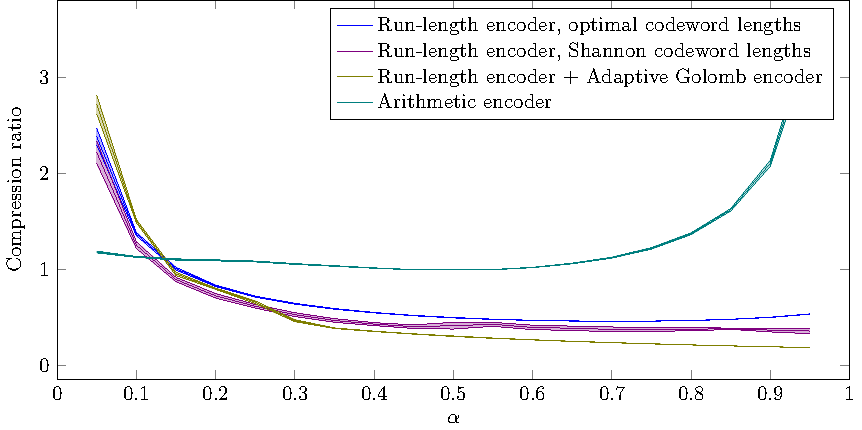
\includegraphics{../tikz/compression_optimal/optimal_run_length.pdf}
  \caption{Compression ratios $\pm\sigma$ of the run-length code for different values of $\alpha$.}
  \label{fig:comprratio}
\end{figure}

\Cref{fig:pmf} plots the statistically measured PMF of the run-length code of the Markov source
for different values of $\alpha$.
The graph is cut short at $x=8$ for increased resolution at the more interesting parts,
but the PMFs continue on for quite long after it with low probabilities
(in the most extreme case to $x=189$ for $\alpha=0.05$).
We can see that the PMF resemble geometric distributions except for the first two values.
This can be explained by the run-length labels that are placed into the code:
for each run-length block the code is placing both the run-length value and the symbol.
Since 1 is used as both a run-length value and a symbol it is more frequently used in the code,
and have therefore a higher probability.

\begin{figure}[!ht]
  \centering
  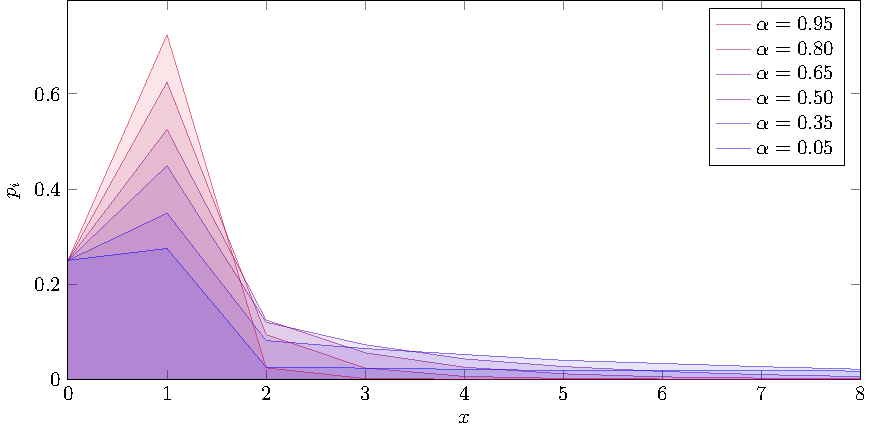
\includegraphics{../tikz/runlength_pmf/runlength_pmf.pdf}
  \caption{PMF of the run-length code symbols for different values of $\alpha$.}
  \label{fig:pmf}
\end{figure}

\section{Q3: Golomb encoder}
\Cref{fig:comprratio} shows the performance of the concatenated run-length and adaptive Golomb encoder.
For some reason it manages to compress the source more efficiently
than both the optimal and Shannon codeword lengths.
I would suspect that I did not accidentaly made a superior code than the theoretical bound
but rather that this result points to something incorrect in my code.

\section{Q4: Arithmetic coding}
For the arithmetic encoder we needed to tailor it to the Markov source.
Since the setup was a binary Markov source with equal switching probabilities for both states
I concatenated switching probabilities to a single probability state
and similarly with the staying probabilities.

The performance of the arithmetic encoder can also be seen in \cref{fig:comprratio}.
It starts off worse than all of the runlength encoders,
but quickly gives better results with increased $\alpha$.
This makes sense since we are not using the run-length version of the source:
when $\alpha$ is high the run-length is not doing a lot of concatenations
since the probability of a state switch is high.
The run-length encoders are therefore performing worse in these stages.

\Cref{fig:entropy} shows the entropy of the Markov source and the encoded string using the Arithmetic encoder.
We can see that the code is quickly reaching the entropy of the source as $\alpha$ increases,
i.e. it gets closer to the theoretical bound of the code performance.

\begin{figure}[!ht]
  \centering
  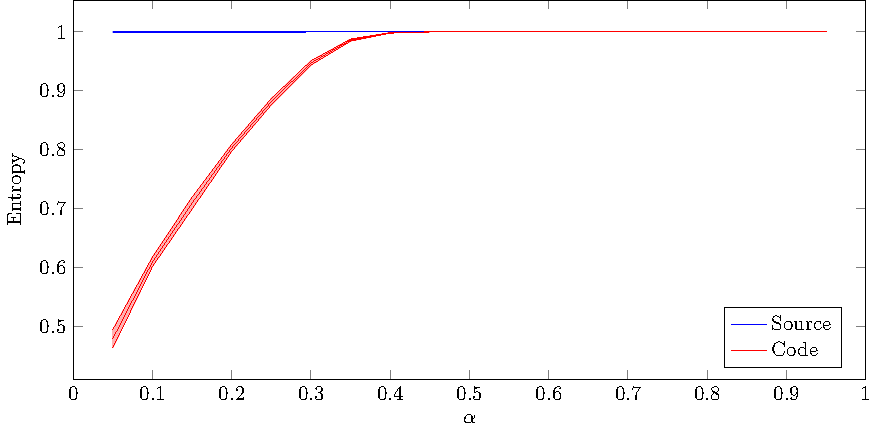
\includegraphics{../tikz/entropy/entropy.pdf}
  \caption{Entropy of the source and the code generated by the arithmetic encoder $\alpha$.}
  \label{fig:entropy}
\end{figure}

\newpage
\section{Appendix}
I wrote that I would add code to the appendix.
However, it ended up being a quite large codebase
and I did not want to typeset all of it.
Instead I put it all on GitHub,
so you can check out all the code at
\href{https://github.com/lbjarre/eq2845-hw3}{https://github.com/lbjarre/eq2845-hw3}.

\end{document}
